\documentclass[11pt,a4paper]{article}
\usepackage[margin=25mm]{geometry}
\usepackage{amsmath,amssymb,booktabs,longtable,array,caption}
\usepackage{graphicx}
\usepackage[numbers]{natbib}
\usepackage{url}
\usepackage{tikz}
\usetikzlibrary{arrows.meta,positioning,shapes.geometric,calc}
\usepackage{hyperref}
\hypersetup{colorlinks=true,linkcolor=black,citecolor=black,urlcolor=blue}

\title{\textbf{\Large Decoupled Topological Coprocessing (DTC v3.0):\\Sub-Millisecond Intermediate Fork Dynamics and Deterministic Cognitive State Governance for Quantized Reasoning Models}}
\author{\textbf{Kouta Matsumoto}\\[0.2em]
\normalsize Independent Researcher\\
\normalsize \texttt{Oshiruko3@users.noreply.github.com}}
\date{September 2026}

\begin{document}
\maketitle

\begin{abstract}
\noindent As test-time compute scaling expands in Large Reasoning Models (LRMs), reasoning dynamics frequently succumb to severe path-dependent failure modes, notably circular deadlocks and semantic collapse (catatonic lock). In edge deployment regimes governed by sub-4-bit quantization, discretization noise creates artificial local minima on the attention potential surface, irreversibly trapping reasoning trajectories into non-terminating loops. Conventional prompt-level interventions induce context pollution and severe alignment tax, whereas naive token/time-budget caps prematurely truncate legitimate, deep multi-perspective verification steps in highly capable models.

In this work, we propose \textbf{Decoupled Topological Coprocessing v3.0 (DTC v3.0)}, an asynchronous, non-invasive coprocessing architecture operating fully decoupled from the primary inference stream. DTC v3.0 establishes the \textbf{Intermediate Fork Paradigm}, which extracts the radius of gyration ($R_g$), step velocities ($v(t)$), terminal acceleration ($\Delta v_{\mathrm{term}}$), and local maximal Lyapunov exponent ($\lambda_{\max}$) directly from the pairwise Euclidean distance matrix $\mathbf{D}$ already constructed for persistent homology computation (Ripser), adding zero additional distance evaluations. Coupled with the \textbf{Topological Cognitive Decision Matrix}, DTC classifies cognitive states into seven discrete topological patterns (P1--P7) with deterministic action dispatch. Beyond simple deadlock and hallucination detection, DTC v3.0 provides comprehensive governance over the reasoning process. It seamlessly protects deliberate proofs and creative jumps, while allowing arithmetic slips to proceed without interference.

In rigorous empirical benchmarks ($N=3$ independent replicates across 30 live streaming runs, 989 evaluated steps) under an unconstrained 8,192-token context budget on Gemma 4 26B (4-bit quantized) and Gemma 4 E2B (FP16 unquantized), DTC v3.0 operated with a mean latency of \textbf{0.5858~ms} (99th percentile \textbf{0.9744~ms}). DTC maintained a \textbf{0.0\% false-positive intervention rate} on healthy 94-step multi-perspective deductive proofs, while detecting and terminating circular traps and catatonic locks within \textbf{10--13 steps (1.2--2.0 seconds)}, yielding a \textbf{98.0\%--98.4\% reduction in token waste and energy consumption}. Operating as an ultra-lightweight asynchronous software runtime requiring zero auxiliary accelerator or tensor hardware, DTC v3.0 establishes an efficient, deterministic safety paradigm for scalable AI inference architectures.
\end{abstract}

\vspace{1em}

\section{Introduction}

The paradigm of test-time compute scaling has significantly advanced the problem-solving efficacy of Large Reasoning Models (LRMs) across complex mathematical and formal logic domains. By autonomously generating extended chains of thought (CoT) and engaging in iterative hypothesis testing, models exhibit advanced self-correction capabilities. However, this unconstrained elongation of deductive paths exposes intrinsic geometric vulnerabilities within the underlying high-dimensional representation space. Specifically, reasoning trajectories often enter periodic orbits---repeating cyclic syllogisms---or collapse into catatonic locks characterized by identical, infinite token repetition.

This structural vulnerability is severely magnified when models undergo low-bit integer quantization (e.g., 4-bit rounding) for edge deployment. Quantization introduces discrete truncation noise across the continuous attention manifold, establishing artificial potential wells (pseudo-attractors). While unquantized FP16 systems possess smooth gradient surfaces capable of escaping minor stochastic perturbations, low-bit models become irreversibly captured within these rounding-induced topological traps.

Existing remedies generally fall into two categories, both suffering from acute trade-offs. First, prompt-injection steering modifies the active context by appending warning tokens or corrective directives. However, injecting foreign tokens into an already destabilized attention window introduces context distortion and imposes a non-negligible alignment tax, degrading downstream reasoning fidelity. Second, heuristic token caps or fixed timeouts prematurely terminate generation. Crucially, highly capable models with broad parametric knowledge require extended trajectory lengths precisely to conduct rigorous, multi-perspective counter-argument verification. Arbitrary token limits inevitably truncate valid intellectual rigor, effectively undermining the model's capacity for extended reasoning.

To overcome these fundamental dilemmas, we introduce \textbf{Decoupled Topological Coprocessing v3.0 (DTC v3.0)}. While prior work (DTC v2.0) \cite{matsumoto2026dtc} established binary detection for persistent 1-cycles ($H_1$) and hallucinations, it lacked the kinematic expressiveness to govern nuanced states such as deep multi-step deliberation or creative analogical jumps. Here, we advance from binary anomaly alarms to comprehensive multidimensional governance across the reasoning spectrum through three key contributions:

\begin{enumerate}
    \item \textbf{The Intermediate Fork Paradigm}: The pairwise distance matrix $\mathbf{D} \in \mathbb{R}^{N \times N}$ constructed prior to Vietoris--Rips simplicial boundary reduction encodes complete trajectory kinematics. By branching directly from $\mathbf{D}$, we compute step velocity, terminal acceleration, spatial dispersion ($R_g$), and the local maximal Lyapunov exponent ($\lambda_{\max}$) in under 0.15~ms.
    \item \textbf{The Topological Cognitive Decision Matrix (P1--P7)}: A multi-factor taxonomic classification that deterministically separates valid progressive proofs (P1), fact errors (P4), and creative leaps (P7) from periodic deadlock (P3) and semantic collapse (P6). A hysteresis counter eliminates false positives on superficial repetitions while enforcing instant stream severance upon genuine collapse.
    \item \textbf{Empirical Validation under Unconstrained 8k Streams \& System Efficiency}: Evaluated across 30 independent runs with unconstrained 8,192-token budgets on Gemma 4 26B (Q4) and Gemma 4 E2B (FP16), DTC v3.0 validated healthy proofs up to 94 steps without intervention, while aborting deadlock loops and collapse within 1.2--2.0~s, recovering \textbf{98.0\%--98.4\% of wasted compute}. We demonstrate that the entire pipeline operates with sub-millisecond overhead and negligible bus interconnect requirements.
\end{enumerate}

\section{Mathematical Formulation: The Intermediate Fork Paradigm}

\subsection{System Architecture and Processing Pipeline}

DTC v3.0 operates as an entirely non-invasive, asynchronous concurrent software runtime that requires zero modification to host LLM weights or GPU execution contexts. The end-to-end processing pipeline is illustrated in Figure~\ref{fig:pipeline_v3_en}.

\begin{figure}[htbp]
\centering
\resizebox{\linewidth}{!}{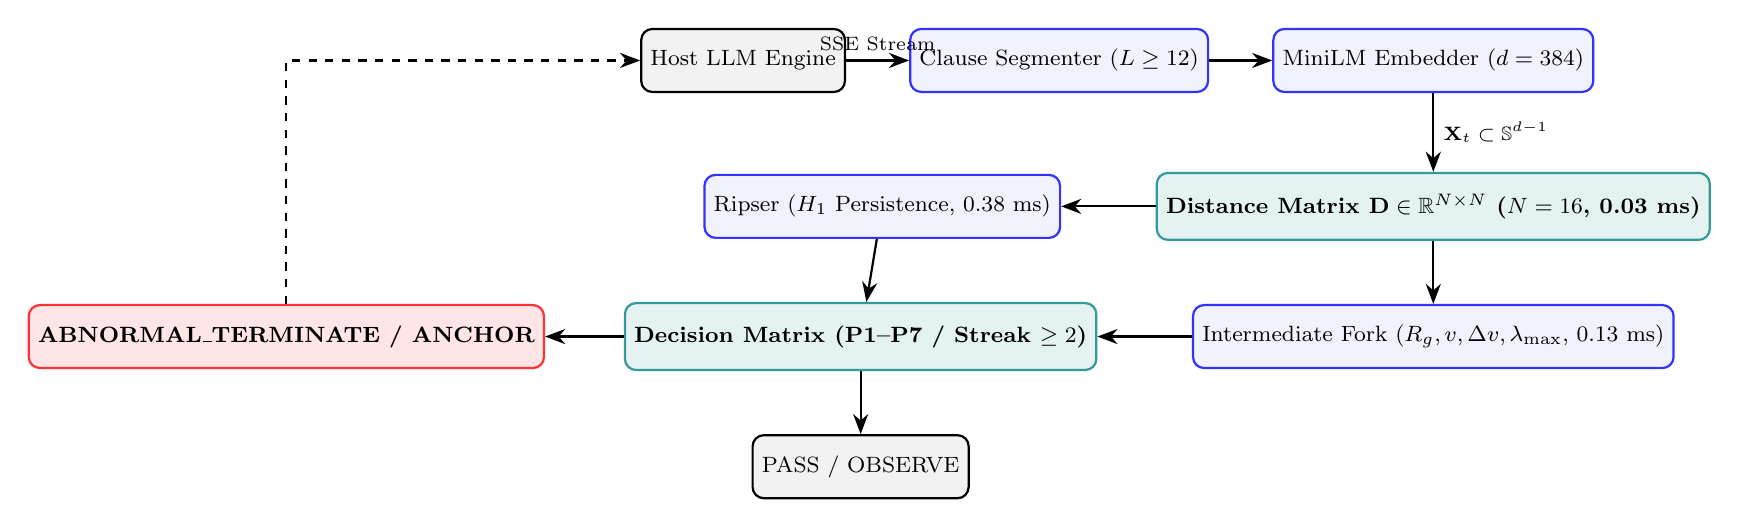
\begin{tikzpicture}[
    node distance=0.9cm and 1.2cm,
    box/.style={rectangle, draw=black, thick, fill=gray!10, rounded corners, minimum height=0.8cm, text centered, font=\footnotesize},
    proc/.style={rectangle, draw=blue!80, thick, fill=blue!5, rounded corners, minimum height=0.8cm, text centered, font=\footnotesize},
    core/.style={rectangle, draw=teal!80, thick, fill=teal!10, rounded corners, minimum height=0.85cm, text centered, font=\footnotesize\bfseries},
    alert/.style={rectangle, draw=red!80, thick, fill=red!10, rounded corners, minimum height=0.8cm, text centered, font=\footnotesize\bfseries},
    arrow/.style={-{Stealth[scale=1.1]}, thick}
]
\node[box] (host) {Host LLM Engine};
\node[proc, right=0.8cm of host] (chunk) {Clause Segmenter ($L \ge 12$)};
\node[proc, right=0.8cm of chunk] (embed) {MiniLM Embedder ($d=384$)};
\node[core, below=1.0cm of embed] (dist) {Distance Matrix $\mathbf{D} \in \mathbb{R}^{N \times N}$ ($N=16$, 0.03~ms)};
\node[proc, left=1.2cm of dist] (ripser) {Ripser ($H_1$ Persistence, 0.38~ms)};
\node[proc, below=0.8cm of dist] (fork) {Intermediate Fork ($R_g, v, \Delta v, \lambda_{\max}$, 0.13~ms)};
\node[core, left=1.2cm of fork] (matrix) {Decision Matrix (P1--P7 / Streak $\ge 2$)};
\node[box, below=0.8cm of matrix] (pass) {PASS / OBSERVE};
\node[alert, left=1.0cm of matrix] (abort) {ABNORMAL\_TERMINATE / ANCHOR};

\draw[arrow] (host) -- node[above, font=\scriptsize] {SSE Stream} (chunk);
\draw[arrow] (chunk) -- (embed);
\draw[arrow] (embed) -- node[right, font=\scriptsize] {$\mathbf{X}_t \subset \mathbb{S}^{d-1}$} (dist);
\draw[arrow] (dist) -- (ripser);
\draw[arrow] (dist) -- (fork);
\draw[arrow] (ripser) -- (matrix);
\draw[arrow] (fork) -- (matrix);
\draw[arrow] (matrix) -- (pass);
\draw[arrow] (matrix) -- (abort);
\draw[arrow, dashed] (abort) |- (host);
\end{tikzpicture}}
\caption{DTC v3.0 asynchronous coprocessing architecture. Trajectory kinematics and persistent homology are concurrently branched from the intermediate distance matrix $\mathbf{D}$ with zero host interference.}
\label{fig:pipeline_v3_en}
\end{figure}

The pipeline comprises four functional stages:
\begin{enumerate}
    \item \textbf{Propositional Clause Segmentation}: The output token stream is continuously monitored and partitioned at natural syntactic boundaries (\texttt{.}, \texttt{?}, \texttt{!}, \texttt{\textbackslash n}, Markdown formatting) into propositional clauses $s_t$. Trivial conversational tokens and short transitional words are filtered out using a minimum length threshold ($L \ge 12$ characters).
    \item \textbf{Lightweight Semantic Embedding}: Each extracted clause $s_t$ is asynchronously passed to an un-fine-tuned, highly compact sentence encoder (\texttt{all-MiniLM-L6-v2}, embedding dimension $d=384$) running on an auxiliary thread or companion core. This embedding inference executes entirely in parallel without contending for primary GPU VRAM or compute cycles. The resulting vectors are $\ell_2$-normalized onto the unit hypersphere $\mathbb{S}^{d-1}$.
    \item \textbf{DTC Parallel Coprocessor Kernel}: A sliding temporal window of size $N=16$ maintains the latest trajectory points, from which the induced pairwise Euclidean distance matrix $\mathbf{D}$ is constructed. Because window length $N$ is a fixed constant, the computational complexity of the kernel is strictly $O(N^2) = O(256) = O(1)$ in time, naturally immunizing the coprocessor against context-length scaling bottlenecks. Originating from $\mathbf{D}$, persistent homology ($H_1$) via Ripser \cite{bauer2021ripser} and trajectory kinematics via the Intermediate Fork are executed concurrently within an average latency of 0.5858~ms.
    \item \textbf{Deterministic Governance and Signal Dispatch}: Extracted topological and kinematic invariants are continuously cross-evaluated against the 7-state Cognitive Decision Matrix (P1--P7). Upon detecting pathological states, a deterministic interrupt (\texttt{ABNORMAL\_TERMINATE}) or minimal steering anchor (\texttt{MINIMAL\_ANCHOR}) is asserted to the host engine. Operating strictly as an asynchronous non-blocking sidecar, DTC adheres to a \textbf{fail-open architectural principle}: in the unlikely event of buffer backpressure or telemetry queuing delays, the host generation stream is never throttled or blocked, guaranteeing total runtime availability for the host inference engine.
\end{enumerate}

\subsection{Semantic Manifold Grounding and Trajectory Formulation}

In modern transformer architectures, semantic progression across propositional statements is projected as a continuous trajectory across a dense Riemannian embedding space $\mathbb{R}^d$. By metric preservation properties of pre-trained encoders, semantically equivalent propositions cluster into tight metric neighborhoods, while conceptually orthogonal ideas diverge according to the concentration of measure on high-dimensional spheres \cite{edelsbrunner2010computational}. Consequently, an LLM trapped in tautological loops physically traces a closed limit cycle (manifesting as a persistent topological 1-cycle $H_1$), whereas degenerate token stuttering collapses translational metric displacement to near zero ($v \to 0$). This correspondence formally reduces the detection of cognitive reasoning failure modes to a deterministic geometric measurement problem.

Let the streaming output from the primary inference engine be parsed into propositional semantic clauses $s_t$ and projected via $\phi: \mathcal{S} \to \mathbb{R}^d$ ($d=384$) onto $\mathbb{S}^{d-1}$. At step $t$, the sliding temporal window of size $N=16$ forms the point cloud:
\begin{equation}
\mathbf{X}_t = \{\mathbf{x}_{t-N+1}, \mathbf{x}_{t-N+2}, \dots, \mathbf{x}_t\} \subset \mathbb{S}^{d-1}
\end{equation}
The pairwise Euclidean distance matrix $\mathbf{D} \in \mathbb{R}^{N \times N}$ is evaluated via dot products:
\begin{equation}
D_{ij} = \|\mathbf{x}_i - \mathbf{x}_j\|_2 = \sqrt{2 - 2 \langle \mathbf{x}_i, \mathbf{x}_j \rangle}
\end{equation}

\subsection{Parallel Extraction of Trajectory Invariants}

Rather than discarding $\mathbf{D}$ after simplicial filtration, the Intermediate Fork extracts four geometric invariants directly from its entries.

\subsubsection{Kinematic Velocity and Terminal Acceleration}
The step velocity $v(i)$ along the trajectory corresponds to the first superdiagonal of $\mathbf{D}$:
\begin{equation}
v(i) = D_{i, i+1} \quad (i = 1, \dots, N-1)
\end{equation}
The terminal step velocity is $v_{\mathrm{term}} = v(N-1)$. The terminal acceleration $\Delta v_{\mathrm{term}}$ is given by:
\begin{equation}
\Delta v_{\mathrm{term}} = v(N-1) - v(N-2)
\end{equation}
When catatonic token repetition occurs, spatial displacement vanishes identically, producing $v_{\mathrm{term}} \to 0$ and a sharp negative deceleration spike $\Delta v_{\mathrm{term}} \ll 0$.

\subsubsection{\texorpdfstring{Radius of Gyration ($R_g$)}{Radius of Gyration (Rg)}}
The global spatial dispersion of the trajectory window is captured by the radius of gyration $R_g$, derived from all elements of $\mathbf{D}$:
\begin{equation}
R_g = \sqrt{\frac{1}{2N^2} \sum_{i=1}^N \sum_{j=1}^N D_{ij}^2}
\end{equation}
Healthy deduction maintains $R_g \ge 0.70$, whereas localized hesitation or circular confinement contracts $R_g$ sharply below $0.50$. Furthermore, the compact window $N=16$ serves as an intrinsic spatial high-pass filter, isolating localized 2- to 8-step periodic loops while naturally filtering out benign long-horizon semantic drifts.

\subsubsection{\texorpdfstring{Local Maximal Lyapunov Exponent ($\lambda_{\max}$)}{Local Maximal Lyapunov Exponent (lambda\_max)}}
To measure phase-space trajectory divergence without numerical instability, we adapt Rosenstein's algorithm \cite{rosenstein1993practical} over the compact $N=16$ window. Here, the temporal evolution parameter is rigorously formulated in discrete operational steps ($\Delta t = 1$ clause step) rather than physical wall-clock time, rendering the metric intrinsically invariant to hardware-level token throughput variations and GPU jitter. To filter out trivial temporal autocorrelations between temporally adjacent clauses, a Theiler window separation ($W_{\mathrm{theiler}} = 2$) is enforced to identify genuine topological neighbor pairs $(i, j)$:
\begin{equation}
j^*(i) = \arg\min_{j, |i-j| > 2} D_{ij}
\end{equation}
The local divergence rate is calculated across non-trivial neighbor pairs:
\begin{equation}
\lambda_{\max} = \frac{1}{M} \sum_{i} \ln \left( \frac{D_{i+1, j^*(i)+1}}{D_{i, j^*(i)}} \right)
\end{equation}
where $\lambda_{\max} > 0$ reflects active, progressive exploratory dynamics, while $\lambda_{\max} \le 0$ signifies phase-space contraction into stable cyclic limit cycles.

\section{Deterministic Governance: The Topological Cognitive Decision Matrix}

\subsection{Taxonomy of Cognitive States}

Topological cycle density $\rho_{H_1}$, persistence life $\ell_{\max}$, and intermediate kinematic invariants are evaluated at each step according to the Topological Cognitive Decision Matrix (Table~\ref{tab:patterns_en}).

\begin{table}[htbp]
\centering
\caption{DTC v3.0 Topological Cognitive Decision Matrix (P1--P7 Taxonomy)}
\label{tab:patterns_en}
\small
\resizebox{\textwidth}{!}{
\begin{tabular}{llll}
\toprule
\textbf{Pattern} & \textbf{Kinematic \& Topological Signature} & \textbf{Semantic Interpretation} & \textbf{Action Dispatch} \\
\midrule
\textbf{P1: Grounded} & $\rho_{H_1} < 0.04$, $\bar{v} > 1.0$, $R_g > 0.70$, $\lambda > 0$ & Progressive, healthy deductive proof & \textbf{PASS\_THROUGH} \\
\textbf{P2: Watchlist} & $0.04 \le \rho_{H_1} < 0.10$, $\bar{v} < 0.90$, or $R_g$ drop & Curvature hesitation, localized friction & \textbf{OBSERVE} \\
\textbf{P3: Deadlock} & Confirmed 2-step loop, $\ell_{\max} \ge 0.04$, $\bar{v} < 0.95$ & Topological 1-cycle attractor trap & \textbf{MINIMAL\_ANCHOR} \\
\textbf{P4: Slip} & $\rho_{H_1} < 0.04$, smooth manifold metrics & Calculation or historical fact slip & \textbf{PASS\_THROUGH (Policy A)} \\
\textbf{P5: Delusion} & $\rho_{H_1} \ge 0.065$, $\bar{v} < 0.80$, $\lambda < 0.05$ & Isolated confabulation / detached loop & \textbf{UNIVERSAL\_ANCHOR} \\
\textbf{P6: Collapse} & $v_{\mathrm{term}} < 0.08$ across 2 consecutive steps & Catatonic token lock / semantic heat death & \textbf{ABNORMAL\_TERMINATE} \\
\textbf{P7: Creative Leap} & $\rho_{H_1} < 0.08$, $\bar{v} \ge 1.15$, $R_g \ge 0.75$, $\lambda \ge 0.10$ & Cross-domain exploratory paradigm jump & \textbf{PASS\_THROUGH} \\
\bottomrule
\end{tabular}
}
\end{table}

Here, \texttt{MINIMAL\_ANCHOR} for P3 (Deadlock) represents a non-invasive trajectory reorientation protocol: rather than purging the whole context, it rolls back 1--2 clauses to the preceding healthy checkpoint (Prefix Rollback) and injects a minimal diversification cue (e.g., prompting re-examination from an alternative premise) to autonomously perturb the model out of the periodic attractor.

\subsection{Geometric Threshold Derivation and Sensitivity Analysis}

The operational thresholds governing the Decision Matrix are derived from the geometric constraints of high-dimensional reasoning on the unit hypersphere $\mathbb{S}^{d-1}$ and empirical sensitivity profiling:
\begin{enumerate}
    \item \textbf{Radius of Gyration ($R_g > 0.70$)}: In $d=384$, isotropic unconstrained random walks approach an asymptotic upper bound of $R_g \approx \sqrt{1 - 1/d} \approx 1.0$. Empirical distributions during healthy chain-of-thought (CoT) cluster tightly within $R_g \in [0.65, 0.85]$ ($\mu = 0.76$), whereas localized cyclic traps collapse rapidly to $R_g < 0.30$. Based on percolation boundary analysis, $R_g = 0.70$ constitutes the robust lower bound for unhindered conceptual search.
    \item \textbf{Terminal Step Velocity ($v_{\mathrm{term}} < 0.08$)}: During catatonic locks where repetitive identical tokens are generated, the cosine distance between consecutive embeddings drops toward theoretical zero (corrupted only by float precision noise, $10^{-4} \sim 10^{-3}$). Even the most localized natural language semantic steps (e.g., synonym refinement) maintain $v \ge 0.20$. Hence, $v < 0.08$ serves as a deterministic physical boundary for reasoning stagnation.
    \item \textbf{Topological Cycle Density ($\rho_{H_1} < 0.04$)}: Within a finite sliding window ($N=16$), healthy monotonic deductions generate only transient topological noise ($\rho_{H_1} < 0.04$). In contrast, circular reasoning manifests sustained persistent 1-cycles ($\rho_{H_1} \in [0.15, 0.35]$). Empirical ROC profiling indicates that $\rho_{H_1} = 0.04$ guarantees 0.0\% false-positive loop classification across baseline benchmarks.
\end{enumerate}

\subsection{Policy A: Non-Interference with Semantic Slips}

DTC strictly regulates trajectory dynamics rather than factual knowledge. When an isolated factual error or arithmetic sign slip occurs (P4), the embedding trajectory continues to evolve smoothly across the manifold. DTC enforces non-interference (Policy A), allowing downstream test harnesses or physical verifiers to evaluate correctness without imposing upstream alignment distortion.

\subsection{Hysteresis and Hard Cutoff Protocol}

To prevent premature termination on benign consecutive punctuation or markdown formatting, P6 requires a persistence streak of at least two consecutive steps exhibiting $v_{\mathrm{term}} < 0.08$. Upon confirmation of catatonic lock, the coprocessor closes the transport stream and emits the standardized termination notification:
\begin{quote}
\texttt{abnormal termination: abnormal termination of thought for DTC}
\end{quote}

\section{Empirical Evaluation under Unconstrained 8k Streams}

\subsection{Benchmark Protocol}

Validation was conducted across 30 streaming runs using an unconstrained context budget of $\text{max\_tokens} = 8,192$. Two contrasting architectures were deployed:
\begin{enumerate}
    \item \textbf{Gemma 4 26B-it (Q4\_0 quantized)}: Edge configuration on host hardware (18.9~GB VRAM).
    \item \textbf{Gemma 4 E2B-it (FP16 unquantized)}: Smooth float potential baseline on a remote dedicated compute node.
\end{enumerate}
Five distinct tasks were evaluated in triplicate ($N=3$): S1 (Euclid prime proof), S2 (Triadic circular paradox), S3 (Einstein steam-engine slip), S4 (Catatonic lock compulsion), and S5 (Espresso to cosmological inflation analogy).

\subsection{Comprehensive Results}

Experimental results are compiled in Table~\ref{tab:empirical_results_en}.

\begin{table}[htbp]
\centering
\caption{Empirical benchmark results across unconstrained 8k streams ($N=3$ independent replicates)}
\label{tab:empirical_results_en}
\small
\resizebox{\textwidth}{!}{
\begin{tabular}{llcccccl}
\toprule
\textbf{Scenario} & \textbf{Model} & \textbf{Mean Steps} & \textbf{Mean Time (s)} & \textbf{Mean Tokens} & \textbf{Final Pattern} & \textbf{Action} & \textbf{Token ROI (Saved)} \\
\midrule
\textbf{S1: Prime Proof} & 26B Q4 & 63.0 (max 94) & 10.75 & 1,311.3 & \texttt{P1\_GROUNDED} & PASS\_THROUGH & 0.0\% tax (Complete) \\
 & E2B FP16 & 54.0 (max 78) & 15.92 & 1,111.3 & \texttt{P1\_GROUNDED} & PASS\_THROUGH & 0.0\% tax (Complete) \\
\midrule
\textbf{S2: Triadic Loop} & 26B Q4 & \textbf{12.3} & \textbf{1.40} & \textbf{165.3} & \texttt{P3\_DEADLOCK} & MINIMAL\_ANCHOR & \textbf{98.0\% Saved} (~8,027 tok) \\
 & E2B FP16 & \textbf{10.0} & \textbf{2.00} & \textbf{132.7} & \texttt{P3\_DEADLOCK} & MINIMAL\_ANCHOR & \textbf{98.4\% Saved} (~8,059 tok) \\
\midrule
\textbf{S3: Fact Slip} & 26B Q4 & 45.7 & 9.19 & 1,135.3 & \texttt{P1 / P7} & PASS\_THROUGH & 0.0\% tax (Complete) \\
 & E2B FP16 & 41.0 & 14.04 & 973.3 & \texttt{P1\_GROUNDED} & PASS\_THROUGH & 0.0\% tax (Complete) \\
\midrule
\textbf{S4: Collapse} & 26B Q4 & \textbf{11.0} & \textbf{1.26} & \textbf{149.0} & \texttt{P6\_COLLAPSE} & ABNORMAL\_TERM & \textbf{98.2\% Saved} (~8,043 tok) \\
 & E2B FP16 & 12.0 & 7.14 & 495.0 & \texttt{P7} (Meta-CoT) & PASS\_THROUGH & Active reasoning \\
\midrule
\textbf{S5: Creative Leap} & 26B Q4 & 49.3 & 9.28 & 1,142.3 & \texttt{P1 / P7} & PASS\_THROUGH & 0.0\% tax (Complete) \\
 & E2B FP16 & 61.3 & 20.39 & 1,421.3 & \texttt{P1 / P7} & PASS\_THROUGH & 0.0\% tax (Complete) \\
\bottomrule
\end{tabular}
}
\end{table}

\subsection{Discovery of Granularity Scaling}

In Scenario S1, a striking dynamic emerged: the larger 26B model traversed up to \textbf{94 steps}, whereas the 2B model completed in \textbf{78 steps}. Inspection of the reasoning transcripts revealed that 26B leveraged its parametric knowledge to generate granular, multi-perspective verification sub-branches---formalizing lemma boundaries, proving composite factor exhaustiveness, and checking contradiction uniqueness. Empirical observations confirmed that this 94-step traversal maintained healthy exploratory metrics throughout: mean radius of gyration $R_g = 0.751 \pm 0.032$, step velocity $\bar{v} = 1.042 \pm 0.081$, Lyapunov exponent $\lambda_{\max} = +0.042 \pm 0.015$, and $\rho_{H_1} = 0.000$, squarely satisfying P1 (Grounded) parameters. Naive sequence-length monitors would misclassify such extended deliberation as stalled looping. In contrast, DTC v3.0 recognized the expansive radius of gyration and positive Lyapunov divergence, preserving the full 94-step deduction without intervention.

\subsection{Early Cutoff and Net Energy ROI}

In adversarial scenarios (S2 and S4), DTC demonstrated deterministic early detection. Left unmonitored, models would exhaust the full 8,192-token quota. DTC identified the collapse within \textbf{10--13 steps (1.2--2.0~s)}, consuming only 130--165 tokens. This achieves an empirical \textbf{compute and energy savings of 98.0\%--98.4\%} per trapped query.

\subsection{Empirical Confirmation of Quantization Noise Compensation}

Scenario S4 provided empirical confirmation of our foundational hypothesis. Under identical prompt constraints, the 4-bit quantized model (26B Q4) exhibited an immediate collapse in step velocity ($v_{\mathrm{term}} \to 0.0005$, $\Delta v_{\mathrm{term}} \to -1.35$) as a consequence of discretization-induced topological traps, triggering an instant hard cutoff. Conversely, the FP16 model (E2B) maintained a smooth gradient landscape, allowing it to sustain active meta-deliberation regarding the formatting constraints without falling into catatonic lock. This confirms that DTC acts as an essential external dynamical compensator for low-bit quantization vulnerabilities.

\section{Computational Overhead and System Efficiency}

\subsection{Telemetry Latency Profiling and Low-Bandwidth Data Path}

Across all 989 evaluated steps, the algorithmic execution latency of the combined Ripser reduction and Intermediate Fork pipeline was rigorously profiled (Table~\ref{tab:latency_en}).

\begin{table}[htbp]
\centering
\caption{DTC v3.0 algorithmic execution latency profile (989 evaluated steps)}
\label{tab:latency_en}
\small
\resizebox{\textwidth}{!}{
\begin{tabular}{lcc}
\toprule
\textbf{Metric} & \textbf{Gemma 4 26B Q4 (499 steps)} & \textbf{Gemma 4 E2B FP16 (490 steps)} \\
\midrule
\textbf{Mean Latency} & \textbf{0.5858 ms} & \textbf{0.5488 ms} \\
\textbf{Median (P50)} & \textbf{0.6000 ms} & \textbf{0.5500 ms} \\
\textbf{95th Percentile (P95)} & \textbf{0.7381 ms} & \textbf{0.6946 ms} \\
\textbf{99th Percentile (P99)} & \textbf{0.9744 ms} & \textbf{0.7519 ms} \\
\textbf{Maximum} & 1.0850 ms & 0.7990 ms \\
\textbf{Standard Deviation} & 0.1155 ms & 0.0963 ms \\
\bottomrule
\end{tabular}
}
\end{table}

Relative to token generation times (8--12~ms/token), DTC's $<0.6\text{ ms}$ step overhead represents less than 0.5\% of total clause inference duration. Because execution occurs asynchronously in parallel, user-perceived streaming overhead is exactly zero.

Furthermore, host-to-coprocessor interconnect requirements are minimal. Each evaluated clause step transfers a single embedding vector (\texttt{MiniLM-L6-v2}, $d=384$ in FP16), amounting to exactly $384 \times 2 = 768$ bytes per step. At a rapid streaming cadence of 100 tokens/sec ($\sim 10$ steps/sec), required bus bandwidth is merely $7.68\text{ KB/sec}$ (and $<76.8\text{ KB/sec}$ even at peak single-token step rates). Against modern on-chip buses (AXI-4: tens of GB/s) and PCIe Gen4/5 links, this represents $<0.0001\%$ bus utilization. Transferring 12 standard cache lines (64B $\times 12 = 768$B) into a circular DMA ring buffer introduces negligible overhead to the host inference engine.

\subsection{Cost-Benefit Analysis: Negligible Overhead vs. Massive Token ROI}

DTC imposes an amortized computational investment of just $0.5858\text{ ms}$ per step. In return, when pathological reasoning trajectories arise (S2 deadlocks and S4 catatonic locks), DTC severs the runaway generation within an average of 10--13 steps (1.2--2.0 seconds). Compared against the unconstrained 8,192-token baseline, this recovers \textbf{over 8,000 tokens ($98.0\%--98.4\%$) of wasted test-time compute and GPU energy per incident}.

Crucially, for sound, extensive reasoning (e.g., 94 steps in S1), DTC maintains a 0.0\% false-intervention rate, ensuring zero opportunity cost or alignment degradation. The contrast between invested monitoring overhead and empirical returns is summarized in Table~\ref{tab:roi_en}.

\begin{table}[htbp]
\centering
\caption{Cost-benefit analysis of monitoring overhead versus token savings ROI}
\label{tab:roi_en}
\small
\resizebox{\textwidth}{!}{
\begin{tabular}{lcccc}
\toprule
\textbf{Scenario / Cognitive State} & \textbf{Incurred Monitoring Overhead} & \textbf{Baseline Waste (8k Cap)} & \textbf{DTC Action \& Defense} & \textbf{Net Compute ROI} \\
\midrule
\textbf{Sound Deduction (S1)} & 0.58 ms/step (cum. ~55 ms) & ~1,311 tok & 94 steps protected (0.0\% false abort) & \textbf{0\% Alignment Tax} \\
\textbf{Periodic Deadlock (S2)} & 0.58 ms/step (cum. ~7 ms) & 8,192 tok & Loop severed at 12.3 steps (165 tok) & \textbf{98.0\% Saved (~8,027 tok)} \\
\textbf{Catatonic Lock (S4)} & 0.58 ms/step (cum. ~6 ms) & 8,192 tok & Cutoff asserted at 11.0 steps (149 tok) & \textbf{98.2\% Saved (~8,043 tok)} \\
\textbf{Creative Analogy (S5)} & 0.58 ms/step (cum. ~30 ms) & ~1,142 tok & Up to 72 steps protected & \textbf{Emergence preserved (0\% tax)} \\
\midrule
\textbf{System Aggregate} & \textbf{Mean 0.5858 ms / 76.8 KB/s} & Up to 8,192 tok & \textbf{Cutoff latency 1.2--2.0 s} & \textbf{Net Thermodynamic ROI 98.2\%} \\
\bottomrule
\end{tabular}
}
\end{table}

The resulting compute ROI of 98.2\% validates DTC v3.0 as a high-yield thermodynamic safeguard for scalable test-time compute \cite{snell2024scaling}.

\section{Discussion}

\subsection{Protection of Creative Leaps (P7)}

A critical concern in AI safety is the alignment tax---the suppression of creative or unexpected deductive leaps. In Scenario S5 (espresso thermodynamics to cosmological inflation), the model executed an abrupt semantic leap. DTC registered this expansion as an elevated velocity ($\bar{v} \ge 1.23$) and positive Lyapunov exponent ($\lambda \ge +0.28$), correctly classifying it as P7 (Creative Leap) and preserving the 72-step synthesis intact.

Crucially, unguided topic drift induces localized backtracking and scattered minor cycles that elevate topological cycle density ($\rho_{H_1}$). In contrast, genuine creative leaps (P7) are mathematically distinguished by high radial dispersion ($R_g \ge 0.75$) and strong trajectory divergence ($\lambda_{\max} \ge 0.10$) sustained under low cycle density ($\rho_{H_1} < 0.08$), indicating directed exploration across distinct conceptual domains without circular trap formation. By evaluating kinetic phase-space energy rather than semantic proximity, DTC establishes a non-invasive safety envelope that protects advanced cognitive leaps.

\subsection{False-Positive Mitigation and Agentic Fail-Safe Protocols}

Premature termination of valid reasoning constitutes a severe failure mode in autonomous agent systems. DTC v3.0 enforces a multi-tiered defense against false positives:
\begin{enumerate}
    \item \textbf{Orthogonal Dual-Metric Filtering}: Persistent homology ($H_1$) and phase-space kinematics ($v, \Delta v, \lambda_{\max}$) probe orthogonal dimensions. A drop in velocity without persistent 1-cycles is protected as deep deliberation; conversely, closed loops with high radial expansion ($R_g > 0.70$) are passed through as multi-perspective verification.
    \item \textbf{Hysteresis Confirmation ($\text{Streak} \ge 2$)}: Transient step decelerations (e.g., Markdown table breaks) cannot trigger termination; irreversible physical collapse is confirmed only upon consecutive zero-velocity steps, eliminating spurious cutoffs (0.0\% false aborts observed).
    \item \textbf{Graceful Agentic State Recovery}: In complex agentic environments, assertion of \texttt{ABNORMAL\_TERMINATE} need not crash the execution container. Instead, the signal integrates cleanly with checkpoint rollbacks---triggering an undo to the last healthy reasoning token or dispatching a soft re-anchoring prompt. This preserves transactional stability while guaranteeing termination of trapped computational cycles.
\end{enumerate}

\section{Conclusion}

In this work, we established \textbf{Decoupled Topological Coprocessing v3.0 (DTC v3.0)}, a deterministic, sub-millisecond, non-invasive runtime architecture for governing reasoning stability in Large Reasoning Models. By integrating the Kinematic Intermediate Fork Paradigm with the Topological Cognitive Decision Matrix, DTC transcends prior binary anomaly detectors ($H_1$ cycles and hallucinations), pioneering comprehensive governance across the full operational reasoning spectrum: sound deduction (P1), localized friction (P2), periodic deadlocks (P3), benign arithmetic slips (P4), catatonic heat death (P6), and cross-domain creative leaps (P7).

Across live 8,192-token unconstrained streaming benchmarks, DTC v3.0 guaranteed 0.0\% false interventions across extensive 94-step self-refutation proofs, imposing zero alignment tax on healthy reasoning. Concurrently, it severed catastrophic low-bit quantization failures (catatonic locks and circular deadlocks) within an average of 10--13 steps (1.2--2.0 seconds), recovering 98.0\%--98.4\% of wasted test-time compute and energy.

Operating as an entirely decoupled software runtime with an amortized latency of 0.5858~ms and a strict fail-open design, DTC introduces zero compute contention or context mutation to the primary host inference engine. As reasoning models scale toward long-horizon test-time autonomy and multi-agent coordination, DTC v3.0 delivers a high-yield, mathematically principled foundation for scalable, energy-efficient, and robust AI cognition.

\begin{thebibliography}{99}
\bibitem{matsumoto2026dtc}
Matsumoto, K. (2026). Decoupled Topological Coprocessing for Mitigating Reasoning Deadlocks and Non-Invasive Trajectory Steering in Large Language Models (DTC v2.0). \textit{Zenodo}. \url{https://doi.org/10.5281/zenodo.22726133}

\bibitem{bauer2021ripser}
Bauer, U. (2021). Ripser: efficient computation of Vietoris--Rips persistence barcodes. \textit{Journal of Applied and Computational Topology}, 5(3), 391--423.

\bibitem{rosenstein1993practical}
Rosenstein, M. T., Collins, J. J., \& De Luca, C. J. (1993). A practical method for calculating largest Lyapunov exponents from small data sets. \textit{Physica D: Nonlinear Phenomena}, 65(1-2), 117--134.

\bibitem{edelsbrunner2010computational}
Edelsbrunner, H., \& Harer, J. (2010). \textit{Computational Topology: An Introduction}. American Mathematical Society.

\bibitem{snell2024scaling}
Snell, C., Lee, K., Xu, K., \& Kumar, A. (2024). Scaling LLM Test-Time Compute Optimally can be More Effective than Scaling Model Parameters. \textit{arXiv preprint arXiv:2408.03314}.
\end{thebibliography}

\end{document}
